\chapter{Results}\label{chap:results}
As described in Chapter\ref{chap:design}, we have collected a number of metrics. Using these metrics, we are able to compare the CC UI library to the original Angular components, the various JS framework wrappers, and various other UI libraries. In the following sections we will break down the various metrics and compare the results between the various libraries.

\section{Render Time}
The render time metric will allow us to evaluate the direct performance impact on users once the page has loaded. We will firstly compare the CC UI library to the original Angular components as well as the other JS framework wrappers. This wil allow us to evaluate the performance impact added by the process of conversion to Web Components, as well as the performance impact added by the JS framework wrappers. After this, we will compare the CC UI library to the UI libraries listed in Table~\ref{tab:design:ui-libraries}, allowing us to evaluate the performance of the CC UI library relative UI libraries as a whole.

\subsection{Cow Components}
As mentioned in Chapter~\ref{chap:experimental-setup}, we have measured three components in particular that every UI library contains. These are the Button, Switch, and Input. We have measured the rendering times of 1 instance, 10 instances and 100 instances of this component. The various render times for the cow-components UI libraries with these numbers of components can be seen in figures~\ref{fig:results:render-time-cow-1},~\ref{fig:results:render-time-cow-10}, and~\ref{fig:results:render-time-cow-100} respectively. We'll first take a look at the single-component render times. When we compare the performance of the CC UI library compared to the original Angular components we find a very small performance impact, with the CC UI library even being faster at rendering a Button. Other than the Angular wrapper's button, the wrappers are only slight slower at rendering. From this we can conclude that, although there is a full Angular root running for each component, the performance impact for a single component is minimal. Now taking a look at the render times for 10 and 100 components, we start to see some big differences. The Web Components version is still able to keep up with the original components when it comes to rendering 10 components, but is eclipsed when rendering 100. It seems that the impact of creating a new Angular root for each component does become significant with many components. Additionally, the render times for the various JS frameworks start to differ quite a lot. We see a trend of the React and Vue wrapper growing further away from the Web Components version, with the Angular wrapper moving away even further. It seems that the performance impact for rendering a relatively small amount of components is minimal, while it scales up relatively quickly with a larger number of components. Especially interesting is the fact that picking a JS framework to develop in is very influential, potentially costing a difference of 150ms over Web Components or 50ms over a different framework.

\begin{figure}[h]
	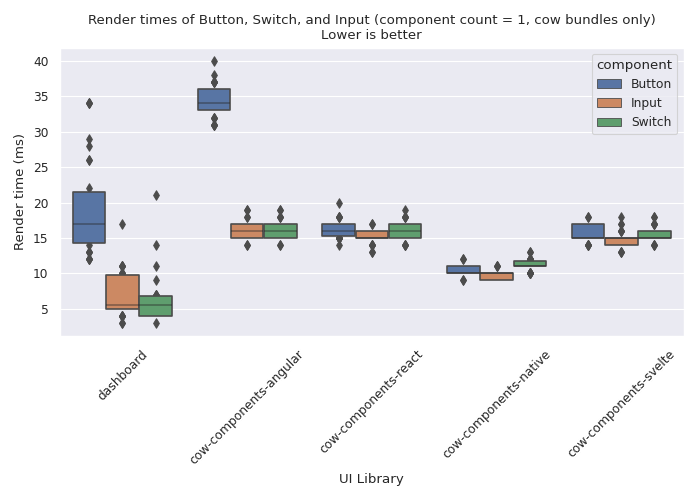
\includegraphics[width=\columnwidth]{plots/render-time-cow-1.png}
	\caption{Render times of a single Button, Switch, or Input component (CC UI only)}
	\label{fig:results:render-time-cow-1}
	\centering
\end{figure}

\begin{figure}[h]
	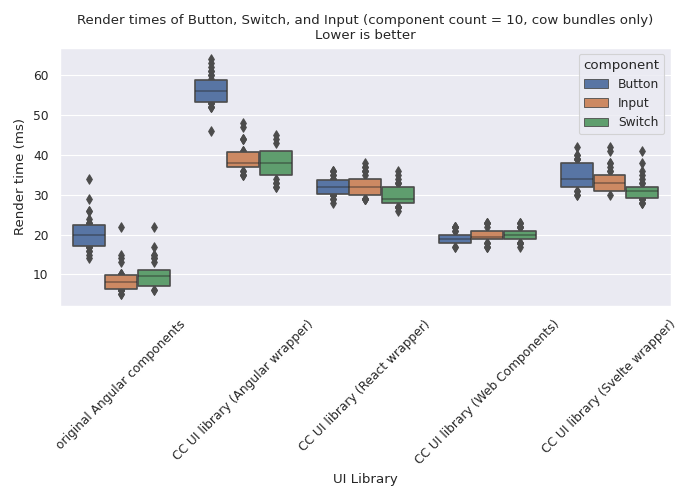
\includegraphics[width=\columnwidth]{plots/render-time-cow-10.png}
	\caption{Render times of ten Button, Switch, or Input components (CC UI only)}
	\label{fig:results:render-time-cow-10}
	\centering
\end{figure}

\begin{figure}[h]
	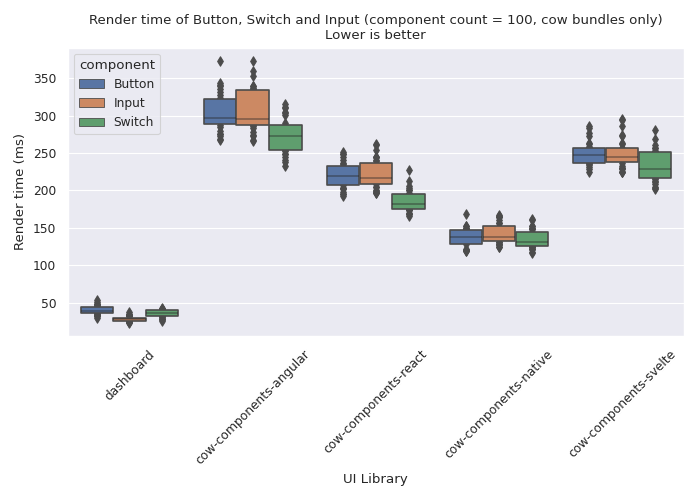
\includegraphics[width=\columnwidth]{plots/render-time-cow-100.png}
	\caption{Render times of one hundred Button, Switch, or Input components (CC UI only)}
	\label{fig:results:render-time-cow-100}
	\centering
\end{figure}

\subsection{UI Libraries}
We now compare the render times of the various UI libraries. Since the number of UI libraries we are comparing is very high (coming in at 29 total), showing them all in one figure makes for a very cluttered view. Instead, we compare a single component at a time. We have chosen to discuss the Button component in this section, however a complete overview can be found in Figures~\ref{fig:appendix:render-time-cow-1},~\ref{fig:appendix:render-time-cow-10}, and~\ref{fig:appendix:render-time-cow-100}. The render times of the Button component for the various UI libraries for 1, 10 and 100 components can be found in figures~\ref{fig:results:render-time-all-1},~\ref{fig:results:render-time-all-10}, and~\ref{fig:results:render-time-all-100} respectively.

We first of all find that there are large differences in render times even within UI libraries that share the same framework. In most cases this has to do with the libraries themselves, but in a few cases this has to do with the type of library. These libraries (\ver{react-bootstrap}, \ver{ng-bootstrap}, and \ver{ngx-bootstrap}) make use of a CSS framework. The idea of a CSS framework is to put most all of the styles a developer will need in a single CSS file. This includes the various variations they could need. For example a CSS library could include the \code{.padding-5} selector as well as the \code{.padding-2} selector for setting the padding of a component. Note that the number of pixels of this padding is included in the selector. This generally leads to relatively big CSS files, which may or may not be treeshaken. This is in contrast to pure UI libraries which generally use per-component stylesheets instead of global stylesheets. They also tend to shift numbers and sizes to JavaScript or HTML\@. For example the same padding as above could be applied through a property, i.e. \code{<my-component padding="2"/>} or \code{<my-component padding="5"/>}. This approach has the advantage of a more per-component focus, more flexibility and options that are easier to discover. However, compared to UI libraries that make use of a CSS framework, normal UI libraries are significantly slower. The UI libraries that make use of a CSS framework generally only append an element to the DOM and apply some pre-computed set of classes to them, meaning they only interact with the very fast JavaScript APIs that are native to the browser. Normal UI libraries on the other hand generally have to run a lot more code.

\begin{figure}[h]
	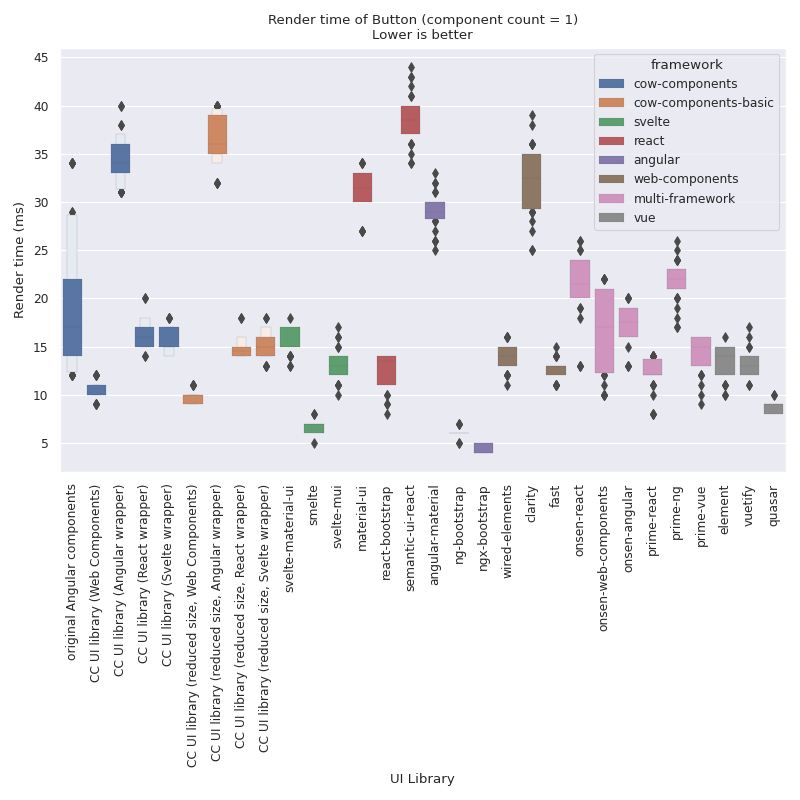
\includegraphics[width=\columnwidth]{plots/render-time-all-1-Button.png}
	\caption{Render times of a single Button. The reduced size CC UI library is the build of the library with less components, as described in Section~\ref{sec:experimental-setup:size}.}
	\label{fig:results:render-time-all-1}
	\centering
\end{figure}

\begin{figure}[h]
	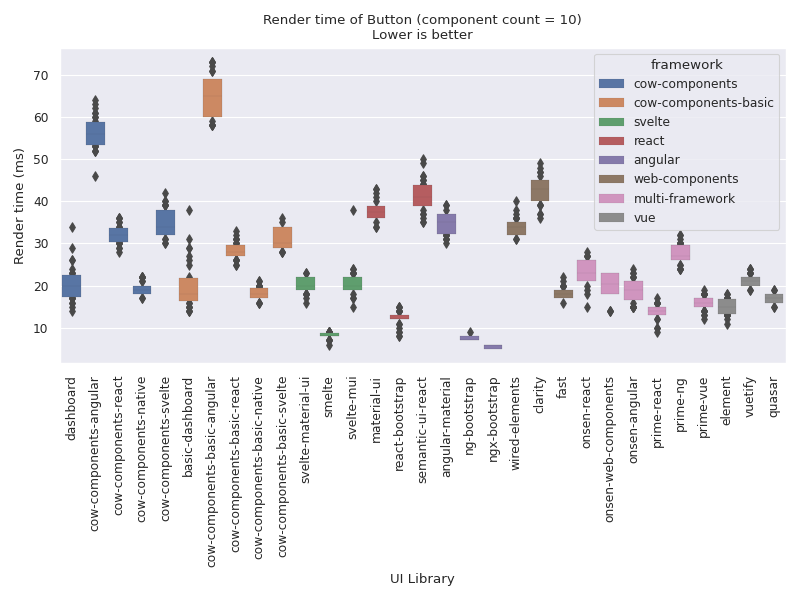
\includegraphics[width=\columnwidth]{plots/render-time-all-10-Button.png}
	\caption{Render times of 10 Buttons. The reduced size CC UI library is the build of the library with less components, as described in Section~\ref{sec:experimental-setup:size}.}
	\label{fig:results:render-time-all-10}
	\centering
\end{figure}

\begin{figure}[h]
	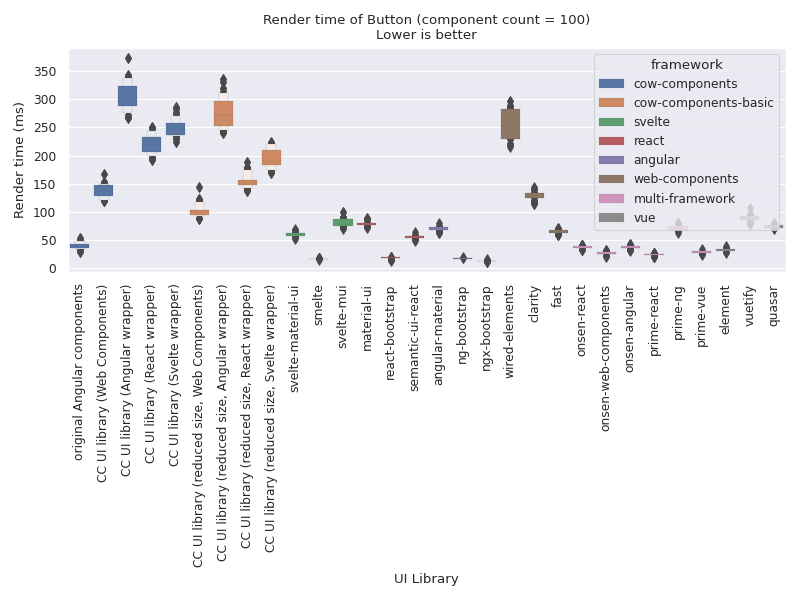
\includegraphics[width=\columnwidth]{plots/render-time-all-100-Button.png}
	\caption{Render times of 100 Buttons. The reduced size CC UI library is the build of the library with less components, as described in Section~\ref{sec:experimental-setup:size}.}
	\label{fig:results:render-time-all-100}
	\centering
\end{figure}

When we ignore these outliers, we can draw some conclusions on the average render times of the various frameworks. We first take a look at the single-component render times in Figure~\ref{fig:results:render-time-all-1}. We can see that Svelte UI libraries are generally very fast. This falls in line with various other performance benchmarks on the internet~\footurl{https://rawgit.com/krausest/js-framework-benchmark/master/webdriver-ts-results/table.html}. After this, Vue and the UI libraries using Web Components are the fastest. It is quite interesting that Web Components are slower than UI libraries using Svelte since Web Components are a native technology, leading one to believe that they would be faster. This might have something to do with the ways in which the authors of the UI libraries created their Web Components. It could be that their approach imposes a significant performance impact. The next frameworks when it comes to render time performance are Angular and React. They are quite close in performance, both being significantly slower than other frameworks. This is again supported by other performance benchmarks on the internet.

We now apply our findings to the CC UI library JS framework wrappers. We find that the performances of our wrappers do not deviate from the general trend we just found. In our case the Web Components version is the fastest simply because every other wrapper builds on top of this version. This means that it is basically impossible for another framework to be faster than it. As expected, the Svelte wrapper is the fastest. Interestingly however, the React wrapper is only slightly slower than the Svelte wrapper, while the Angular wrapper is significantly slower than the both of them. This is in contrast to what we just found, where both Angular and React were slow. It could be that the various internals of React that keep track of state and properties are slow. These are likely to be used a lot by regular React UI libraries which need to handle their state entirely in React, while our React wrapper simply renders a component and passes it its properties once. In general, the CC UI library seems to be able to compete with the render times of other UI libraries, being faster than quite a few of them.

When we start to look at the render times for 10 and 100 components in Figure~\ref{fig:results:render-time-all-10} and Figure~\ref{fig:results:render-time-all-100} however, this trend starts to change. The CC UI libraries seems to not scale well with a large number of components. This confirms our findings in the previous section.

\section{Load Time}
The load time metric will allow us to evaluate the initial performance impact of the CC UI library. Again, we will be comparing the various wrappers to each other as well as the original Angular components. As we will elaborate on later, the Angular wrapper is significantly slower than any other UI library. For this reason we will be splitting every figure into both a figure with and without the Angular wrapper. This should help show the scale of both this large outlier, while not reducing the precision of the scale for other UI libraries.

\subsection{Cow Components}
The load time of the CC UI libraries can be seen in Figure~\ref{fig:results:load-time-cow-no-angular} (without the Angular wrapper) and Figure~\ref{fig:results:load-time-cow} (with the Angular wrapper). When we compare the load time of the CC UI library to the load time of the original 30MHz dashboard, we find that the CC UI library is significantly slower, coming in at about twice the load time. This is likely because the 30MHz dashboard has been optimized specifically for the initial load time. It loads the minimum amount of JavaScript needed to render the page. After this, other files are only loaded on an as-needed basis. The CC UI library on the other hand has to be contained in a single file. Splitting it up into multiple files and instructing 3rd party developers to have multiple JS bundles just to make the CC UI library work would be a terrible developer experience. Concatenating the files into a single big bundle means all of the code has to be parsed and executed, slowing down execution by quite a lot. Comparing the various wrappers to each other, we can first of all see that both the React and Svelte wrappers are just slightly slower than the CC UI library. The added load time is likely to be added by the JS frameworks themselves. Finally, we can see that the Angular wrapper is by far the slowest. This is not entirely unexpected. As mentioned in Section~\ref{sec:case-study:ivy}, we had to disable AOT compilation for the Angular wrapper. This means all Angular compilation happens in the browser instead of during the compilation of the JS bundle. This is likely to be the reason why the Angular wrapper is so slow.

Taking a look at the reduced-size CC UI library, we find the loading times to be only slightly higher than the original components. It appears that a significant portion of the loading was spent in these removed components. Again, the JS framework wrappers are slightly slower, with the Angular wrapper being significantly slower.

\begin{figure}[h]
	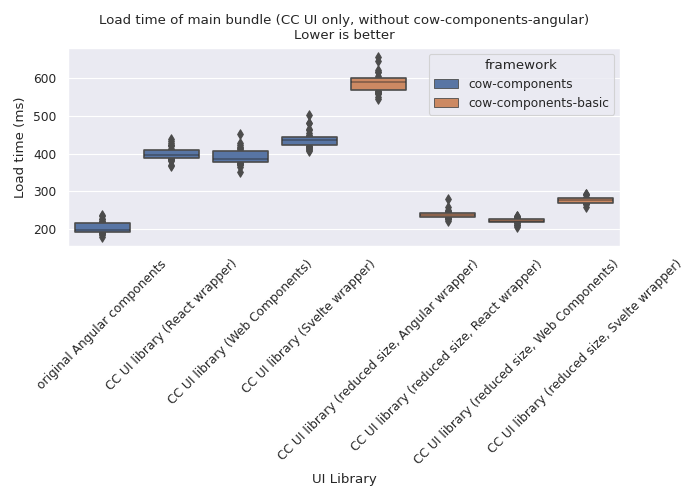
\includegraphics[width=\columnwidth]{plots/load-time-cow-no-angular.png}
	\caption{Load time of the main JS bundle (CC UI only, without Angular wrapper).}
	\label{fig:results:load-time-cow-no-angular}
	\centering
\end{figure}

\begin{figure}[h]
	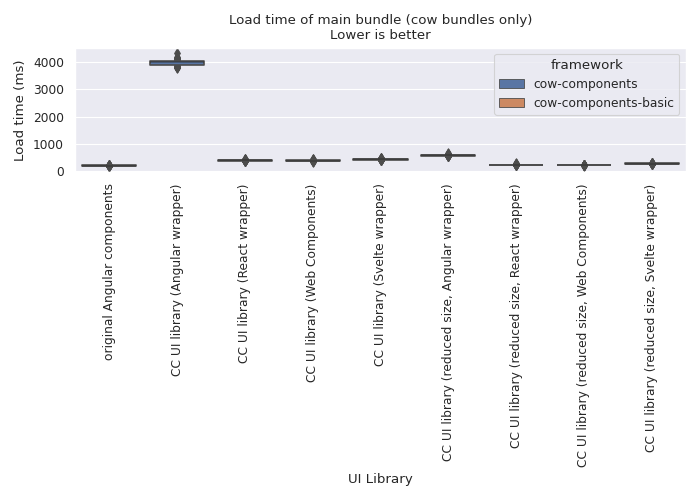
\includegraphics[width=\columnwidth]{plots/load-time-cow.png}
	\caption{Load time of the main JS bundle (CC UI only).}
	\label{fig:results:load-time-cow}
	\centering
\end{figure}

\subsection{UI Libraries}
The load times of other UI libraries can be seen in Figure~\ref{fig:results:load-time-all-no-angular} (without Angular wrapper) and Figure~\ref{fig:results:load-time-all} (with Angular wrapper). It is obvious that other UI libraries largely differ in load time as well. We can first of all see that Svelte UI libraries are by far the fastest, followed closely by Web Components UI libraries and Vue UI libraries. After this, React UI libraries are the fastest. Finally we have Angular, which is by far the slowest. Interestingly, we can see that the different distributions of multi-framework UI libraries follow this same pattern. For example the \ver{prime-ng} UI library is significantly slower than the \ver{prime-react} UI library. Similarly, \ver{onsen-angular} is significantly slower than \ver{onsen-react} and \ver{onsen-web-components}. This could also be one of the factors that is causing our Angular wrapper to be slower, although the lack of AOT compilation is still by far the most influential factor.

As was expected, the CC UI library is quite a bit slower than other UI libraries when it comes to loading. This almost entirely comes down to the tree shaking issue mentioned before. However, loading times of a little over 400ms are not terrible and should be very manageable.

\begin{figure}[h]
	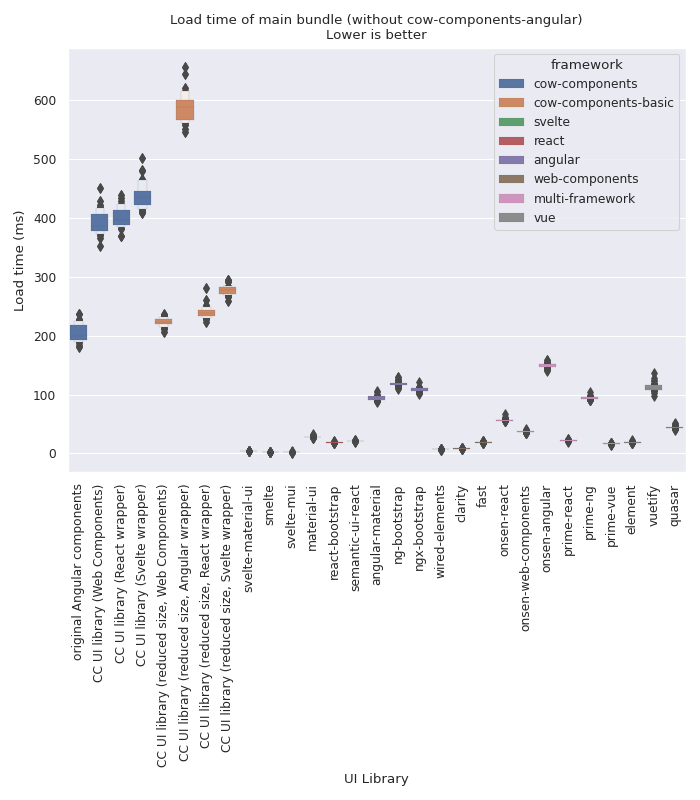
\includegraphics[width=\columnwidth]{plots/load-time-all-no-angular.png}
	\caption{Load time of the main JS bundle (without Angular wrapper).}
	\label{fig:results:load-time-all-no-angular}
	\centering
\end{figure}

\begin{figure}[h]
	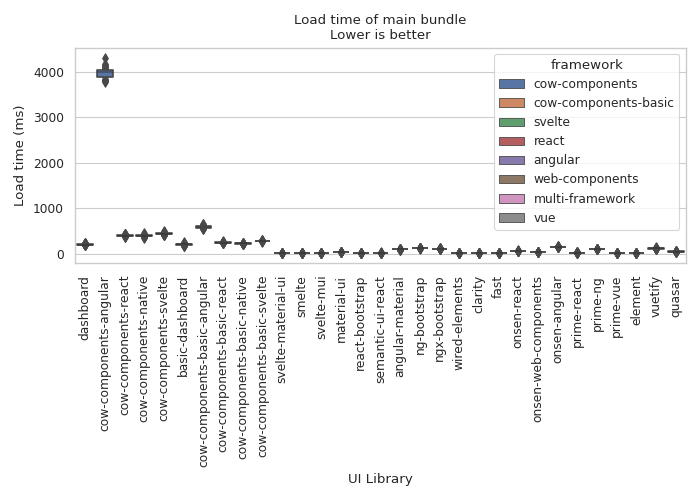
\includegraphics[width=\columnwidth]{plots/load-time-all.png}
	\caption{Load time of the main JS bundle.}
	\label{fig:results:load-time-all}
	\centering
\end{figure}

\section{Bundle Size}
Bundle size is a more abstract representation of the previous metric, allowing us to take a look at the impact of just the bundle size itself. This excludes any performance impact that can be attributed to poorly optimized code. This will also allow us to look at what the performance impact of the Angular wrapper would be if there was no issue with AOT compilation.

\begin{figure}[h]
	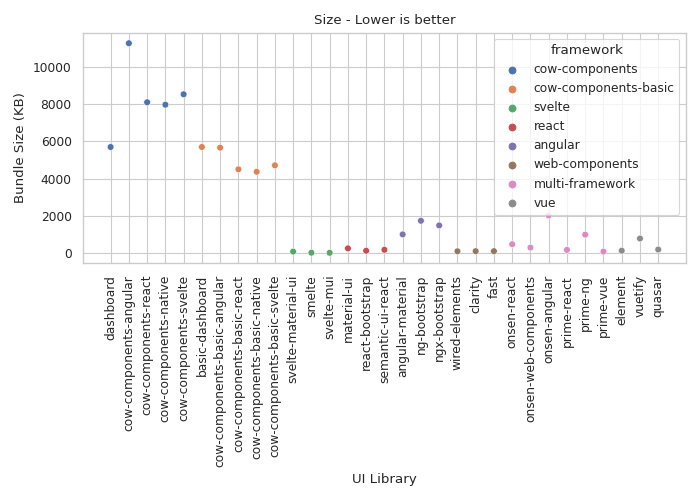
\includegraphics[width=\columnwidth]{plots/size.png}
	\caption{Size of the main JS bundle.}
	\label{fig:results:size}
	\centering
\end{figure}


The various bundle sizes can be seen in Figure~\ref{fig:results:size}. We can first of all see that the bundle sizes correlate strongly with the load times. From this we can conclude that they are a very good representation of the load time metric. We can again see that Svelte, Vue, and Web Component UI libraries are the smallest, with React following closely after them and with Angular being by far the biggest. This is also visible in our various wrappers. The Angular wrapper is by far the biggest. With the strong correlation between load time and bundle size we can conclude that a large part of the Angular wrapper's slow load time can be attributed to the large bundle size.

\section{Page Load Time}
The page load time metric should give us an idea of the real-world loading time of the CC UI library. As described in Chapter~\ref{chap:experimental-setup}, we replicated a page containing all components in the various distributions of the CC UI library. This means that all versions are rendering essentially the same page but in their own framework.

The resulting page load times can be seen in Figure~\ref{fig:results:first-paint}. We have included both the \ver{First Paint} and \ver{First Contenful Paint} metrics, which seem to be almost entirely the same. Interestingly, the Web Components version of the CC UI library loads faster than the equivalent page in the 30MHz dashboard. This is likely because the dasboard has a lot of other tasks going on at runtime, while the CC UI library has been trimmed somewhat to only handle the components. Apart from this, we can see a familiar trend of React and Svelte being slightly slower than the original and Angular being significantly slower.

\begin{figure}[h]
	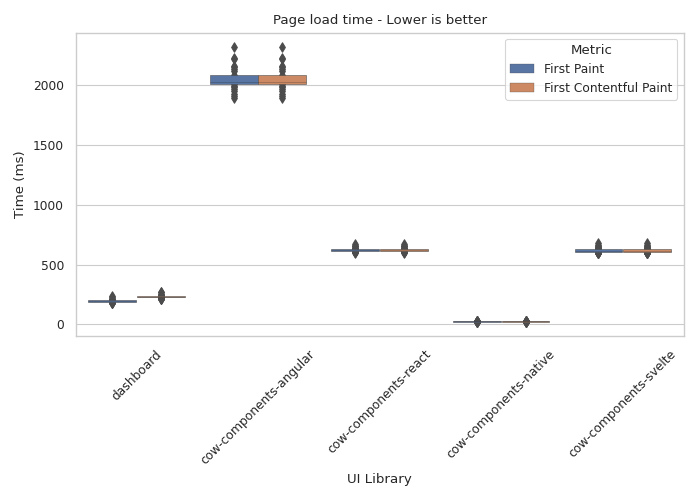
\includegraphics[width=\columnwidth]{plots/first-contentful-paint.png}
	\caption{First paint metrics for the various demo pages.}
	\label{fig:results:first-paint}
	\centering
\end{figure}

\section{Quality of Web Components}
In this section we will be taking a look at the quality of the Web Components in the CC UI library. Note that we are essentially measuring the quality of the original Angular components. This means that the conclusions drawn in this section only apply to the 30MHz codebase and will not be the same for other source codebases.

\begin{figure}[h]
	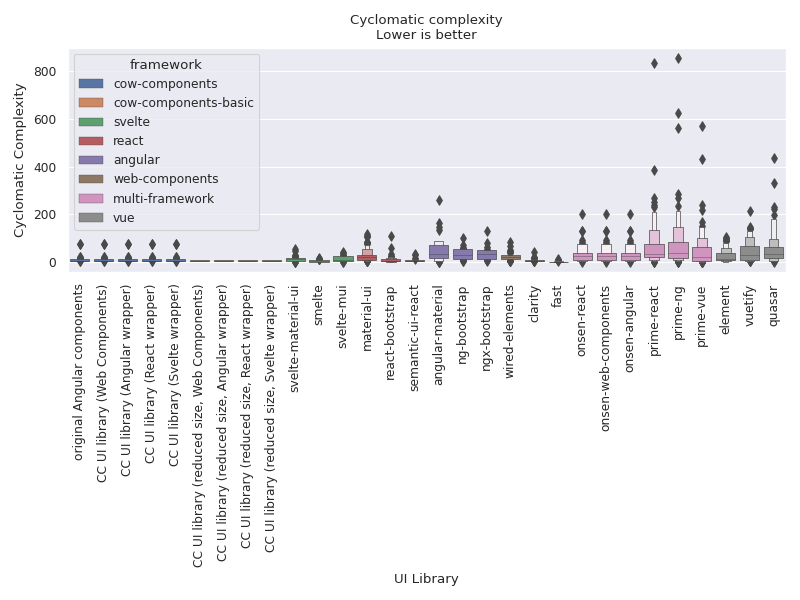
\includegraphics[width=\columnwidth]{plots/cyclomatic-complexity.png}
	\caption{Cyclomatic complexity of the various UI libraries.}
	\label{fig:results:cyclomatic-complexity}
	\centering
\end{figure}

\textbf{Cyclomatic complexity:} The cyclomatic complexities of the various UI libraries can be seen in Figure~\ref{fig:results:cyclomatic-complexity}. It appears that the cyclomatic complexity of the CC UI library is quite good, staying relatively low compared to other UI libraries. It seems that especially multi-framework UI libraries have a very high cyclomatic complexity. This makes sense since these libraries often try to share the source code between the various frameworks as much as possible, leading to a lot of imports.

\begin{figure}[h]
	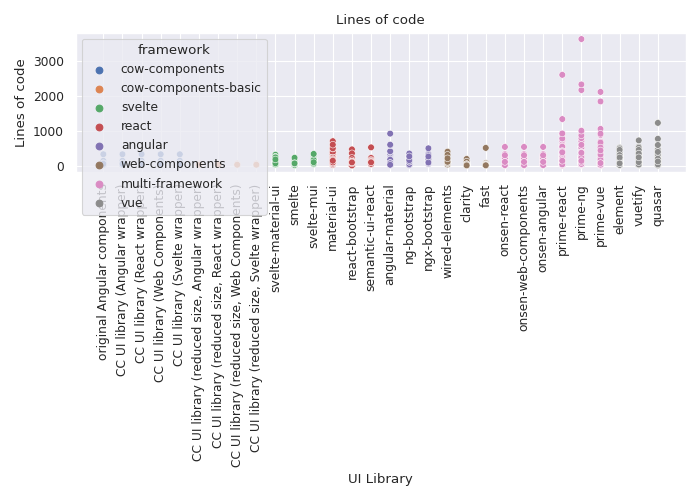
\includegraphics[width=\columnwidth]{plots/lines-of-code.png}
	\caption{Lines of code of the various UI libraries.}
	\label{fig:results:lines-of-code}
	\centering
\end{figure}

\textbf{Lines of code:} The amounts of lines of code can be seen in figure~\ref{fig:results:lines-of-code}. Again we see the same trend of the CC UI library being relatively low in complexity (and as such lines of code), while multi-framework UI libraries have much higher numbers.

\begin{figure}[h]
	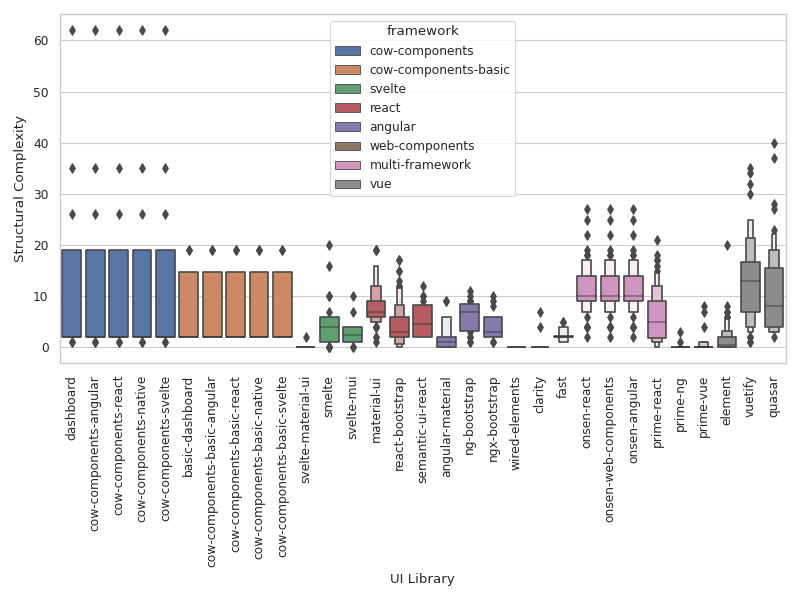
\includegraphics[width=\columnwidth]{plots/structural-complexity.png}
	\caption{Structural complexity of the various UI libraries.}
	\label{fig:results:structural-complexity}
	\centering
\end{figure}

\textbf{Structural complexity:} The structural complexities can be seen in figure~\ref{fig:results:structural-complexity}. This time it appears that the structural complexity of the CC UI library is relatively high. The single measurement at the top is likely to be the Chart component, which is by far the biggest component.

\begin{figure}[h]
	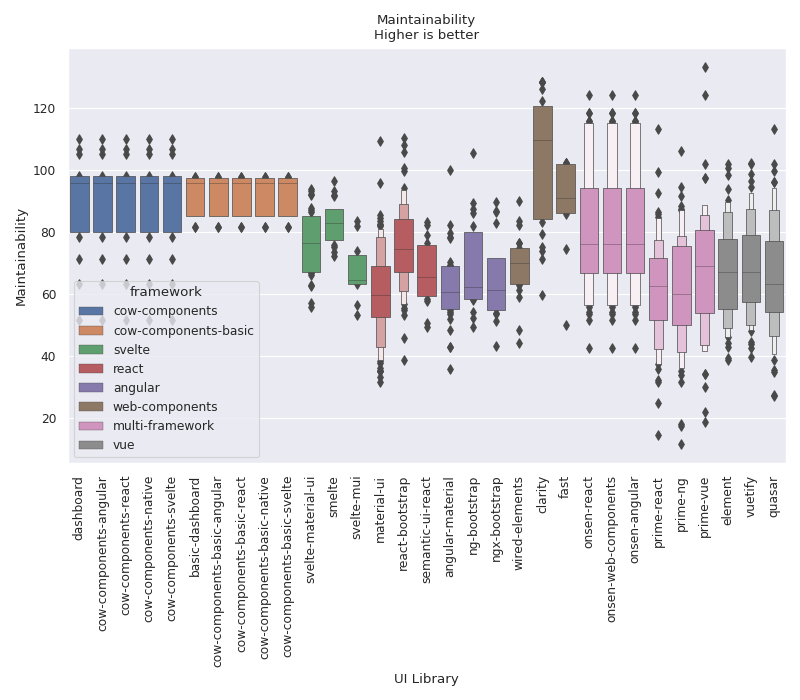
\includegraphics[width=\columnwidth]{plots/maintainability.png}
	\caption{Maintainability of the various UI libraries.}
	\label{fig:results:maintainabilty}
	\centering
\end{figure}

\textbf{Maintainability:} The maintainabilities can be seen in figure~\ref{fig:results:maintainabilty}. It looks like the maintainabilities are a lot more spread out than the previous metrics. It also appears that the CC UI library scores quite well in this metric. Altogether we can conclude that the quality of the CC UI library components (and as such the Angular components they are based off) is quite high.

\section{Time spent on the project}\label{sec:results:time-spent}
While the technical results of this project are important, we also decided to take a look at the business side of this project. An important factor here would be the amount of effort required to complete this project. In total this project took five months of FTE to complete. An estimation would be that about one month was spent on Web Component related issues, three months on Angular related issues and one month on creating JS framework wrappers, and one month on other tasks such as creating a build pipeline, package distributions etc. Note that the time taken is completely separate from the number of components in the resulting UI library, meaning an added component would not increase the time taken at all. Depending on the time required to build the UI library from scratch combined with the time taken maintaining the UI library and adding new components, this project could very well be worth it.